\subsection{Archery}

\begin{enumerate}

\item Essence of Archery
    \begin{itemize}
    \item Paralympic archery is a test of precision, control, and mental focus, where athletes with various impairments compete to hit a target with a bow and arrow. 
    \item It requires incredible concentration and steady hands, as even the slightest movement can affect the trajectory of the arrow. 
    \item To ensure fair competition and enable athletes with different abilities to participate, Paralympic archery incorporates a range of adaptive equipment, including wheelchairs, stools, and mouth tabs for those with limited arm or hand function.
    \end{itemize}

\begin{figure}[htbp] % htbp are float placement options
\centering
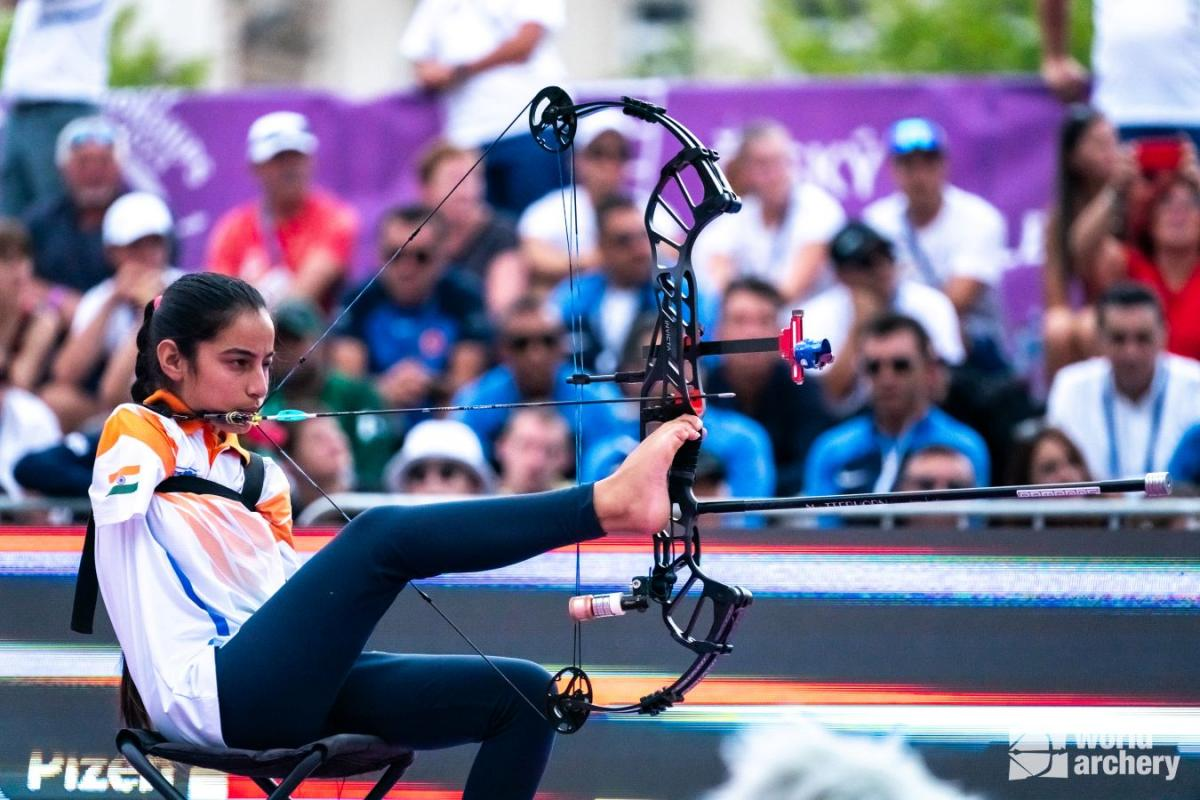
\includegraphics[width=0.8\textwidth]{Images/para_archery.jpg}
\caption{Para Archery}
\label{fig:my_image}
\end{figure}

\item Rules, Equipment, and Competition
    \begin{itemize}
    \item Paralympic archery follows similar rules to Olympic archery, with athletes aiming to score the highest points by hitting the center of a target at various distances. 
    \item Recurve bows and compound bows are the two main types used, and athletes can use assistive devices based on their classification. 
    \item Competition formats include individual, team, and mixed events, adding to the excitement and showcasing the diverse talents of Paralympic archers.
    \end{itemize}

\item Categories and Classifications
    \begin{itemize}
    \item Paralympic archery utilizes a classification system based on the athlete's physical impairment. 
    \item There are three main categories: 
        \begin{itemize}
        \item W1 for athletes with significant limitations in their upper and lower limbs
        \item W2 for those with impairments primarily affecting their lower limbs
        \item Open for athletes with less severe impairments
        \end{itemize}
    \item The classification system ensures that athletes compete against others with comparable functional abilities, fostering fairness and enabling everyone to reach their full potential in the sport.
    \end{itemize}

\end{enumerate}